\begin{frame}{Introduction}
\framesubtitle{IoT}
\begin{columns}
\begin{column}{0.6\textwidth}
\begin{itemize}
  \item 25 billion devices connected
  \item Analytics, management
  \item Multiple Sectors
  \begin{itemize}
    \item Transportation
    \item Smart city
    \item Smart domotics
    \item Smart health
    \item Supply Chain
    \item Agriculture
    \item \ldots
  \end{itemize}
\end{itemize}
\end{column}
\begin{column}{0.4\textwidth}
\begin{figure}
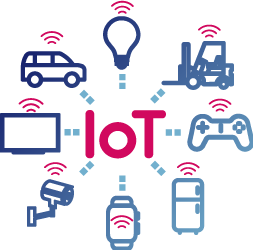
\includegraphics[width=0.8\textwidth]{presentation.tex/fig/iot.png}
\end{figure}
\end{column}
\end{columns}
\end{frame}

\begin{frame}{Introduction}
\framesubtitle{Low Power Wide Area Network (LPWAN)}

\begin{columns}
\begin{column}{0.3\textwidth}
\only<1>{
Short-range
\begin{itemize}
    \item Low power
    \item Small range
    \item Low cost
    \item Low data-rate
    % \item Built for IoT
\end{itemize}
}
\only<2>{
WiFi
\begin{itemize}
    \item Small range
    \item High data-rate
\end{itemize}
}
\only<3>{
Cellular
\begin{itemize}
    \item Long range
    \item High deployement cost
    \item High data-rate
\end{itemize}
}
\only<4>{
LPWAN
\begin{itemize}
    \item Low power
    \item Long range
    \item Low cost
    \item Low data-rate
    \item Built for IoT
    % \begin{itemize}
    %     \item Large scale monitoring
    %     \item Battery operated
    % \end{itemize}
\end{itemize}
}
\end{column}
\begin{column}{0.7\textwidth}

\begin{figure}[H] % TODO More info on axis
\centering
  \resizebox{7.8cm}{4cm}{%
  \begin{tikzpicture}
    \draw[->,thick] (-0.1,0)--(12,0) node[right]{Range};
    \draw[->,thick] (0,-0.1)--(0,8) node[above]{Data Rate};
    \node[] at (1, -0.5) {10m};
    \draw[] (1,-0.1)--(1,0.1);
    \node[] at (3, -0.5) {100m};
    \draw[] (3,-0.1)--(3,0.1);
    \node[] at (5, -0.5) {1km};
    \draw[] (5,-0.1)--(5,0.1);
    \node[] at (7, -0.5) {10km};
    \draw[] (7,-0.1)--(7,0.1);
    \node[] at (9, -0.5) {100km};
    \draw[] (9,-0.1)--(9,0.1);

    \node[] at (-1.2, 1) {1 kbit/sec};
    \draw[] (-0.1,1)--(0.1,1);
    \node[] at (-1.2, 3) {1 Mbit/sec};
    \draw[] (-0.1,3)--(0.1,3);
    \node[] at (-1.2, 5) {100 Mbit/sec};
    \draw[] (-0.1,5)--(0.1,5);
    \node[] at (-1.2, 7) {1 Gbit/sec};
    \draw[] (-0.1,7)--(0.1,7);

    \node[draw,fill=white, visible on=<4->] at (8,1.5) (lora) {LoRa};
    \node[draw,fill=white, visible on=<4->] at (8.7,0.8) (sigfox) {SigFox};
    \node[draw,fill=white, visible on=<4->] at (7.4,2.2) (nb) {NB-IOT};
    \begin{scope}[on background layer]
      \node[draw,fill=blue!30,fit=(lora) (sigfox) (nb), label=above:{LPWAN}, visible on=<4->] {};
    \end{scope}

    \node[draw,fill=white] at (2.2,3.5) (bluetooth) {Bluetooth};
    \node[draw,fill=white] at (2.7,2.5) (zigbee) {ZigBee};
    \node[draw,fill=white] at (2.0,1.8) (ble) {BLE};
    \begin{scope}[on background layer]
      \node[draw,fill=blue!10,fit=(bluetooth) (zigbee) (ble), label=above:{Short-range}] {};
    \end{scope}

    \node[draw,fill=white, visible on=<2->] at (3,5) (wifi) {WiFi};
    \begin{scope}[on background layer]
      \node[draw,fill=blue!50,fit=(wifi), visible on=<2->] {};
    \end{scope}

    \node[draw,fill=white, visible on=<3->] at (6.8,5) (lte) {LTE};
    \node[draw,fill=white, visible on=<3->] at (5.8,6) (5g) {5G};
    \begin{scope}[on background layer]
      \node[draw,fill=blue!60,fit=(lte) (5g), label=above:{Cellular}, visible on=<3->] {};
    \end{scope}

    \node[] at (6.9,8.2) (leg5) {\small Low};
    \node[draw,fill=blue!10] at (7.5,8.2) (leg1) {};
    \node[draw,fill=blue!30] at (7.8,8.2) (leg2) {};
    \node[draw,fill=blue!50] at (8.1,8.2) (leg3) {};
    \node[draw,fill=blue!60] at (8.4,8.2) (leg4) {};
    \node[] at (10.7,8.2) (leg5) {\small High Power Consumption};
\end{tikzpicture}
  }
\caption{Comparison of IoT technologies}
\label{fig:commrangegraph}
\end{figure}
\end{column}
\end{columns}
\end{frame}

\begin{frame}{Introduction}
\framesubtitle{LoRa}
\begin{itemize}
  \item 
\end{itemize}
\end{frame}

\begin{frame}{Introduction}
\framesubtitle{LoRaWAN}
\begin{columns}
\begin{column}{0.5\textwidth}
\begin{itemize}
    \item Stars-of-stars topology
\end{itemize}
\end{column}
\begin{column}{0.5\textwidth}
\begin{figure}
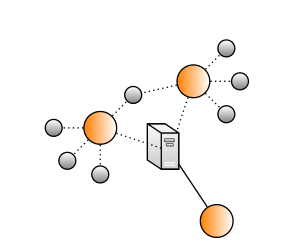
\includegraphics[width=1\textwidth]{presentation.tex/fig/starsofstars.png}
\end{figure}
\end{column}
\end{columns}
\end{frame}


